\section{Introduction to Convolutional Neural Networks}
\begin{frame}{}
    \LARGE CNN: \textbf{Introduction to Convolutional Neural Networks}
\end{frame}

\begin{frame}[allowframebreaks]{Why Do We Need Special Models for Images?}
    Images are grids/matrix of numbers!
    \begin{figure}
        \centering
        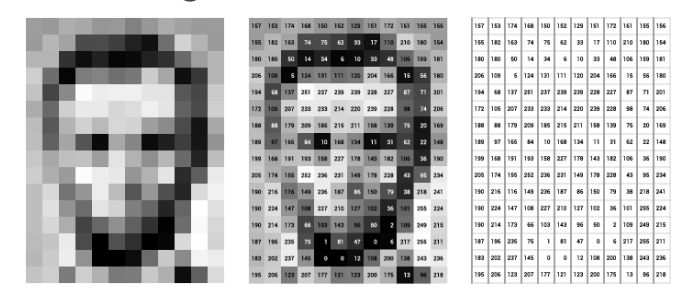
\includegraphics[height=0.8\textheight,width=1\textwidth,keepaspectratio]{images/cnn/represent_image.png}
    \end{figure}
    Images are \textbf{BIG} (e.g., $256 \times 256 \times 3 \approx 200,\!000$ numbers)
    \framebreak
    
    \begin{columns}
        \begin{column}{0.35\textwidth}
            \textbf{Fully Connected Neural Networks:} \\[2em]
            \begin{itemize}
                \setlength{\itemsep}{1em}
                \item Too many parameters
                \item Miss spatial information
            \end{itemize}
        \end{column}
        \begin{column}{0.75\textwidth}
            \begin{figure}
                \centering
                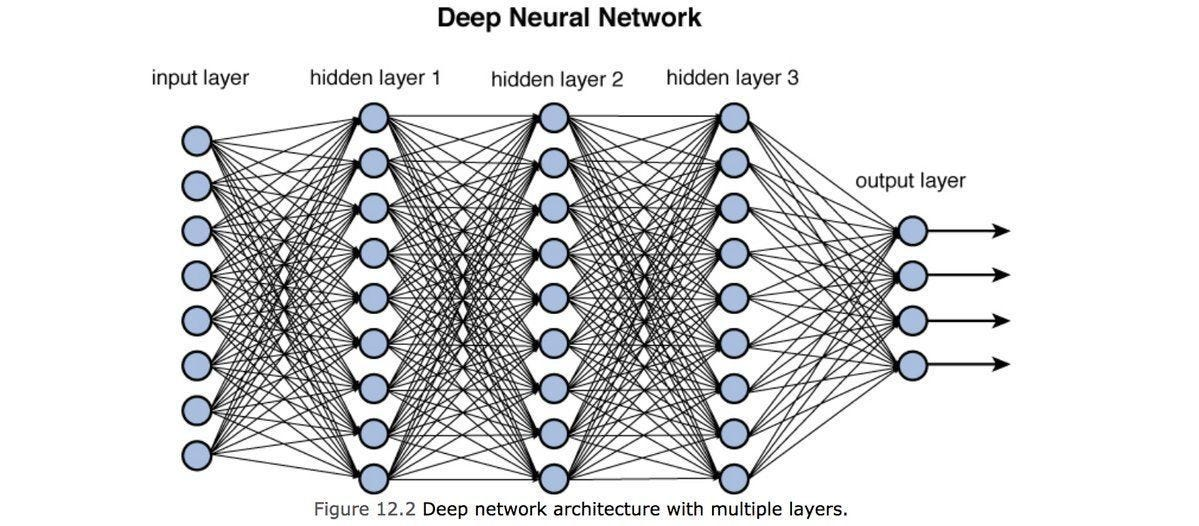
\includegraphics[height=0.8\textheight,width=1.05\textwidth,keepaspectratio]{images/cnn/nn.jpg}
            \end{figure}

            $$z = W_1x_1 + W_2x_2 + \cdots + W_n x_n + b$$
            \footnote{\url{https://towardsdatascience.com/training-deep-neural-networks-9fdb1964b964}}
        \end{column}
    \end{columns}
\end{frame}

\begin{frame}[allowframebreaks]{Drawbacks of Fully-Connected Neural Networks}
    \begin{itemize}
        \item The number of trainable parameters becomes extremely large
    \end{itemize}

    \begin{figure}
    \centering
    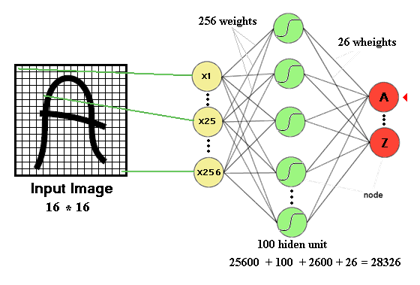
\includegraphics[width=1.0\textwidth,height=0.8\textheight,keepaspectratio]{images/cnn/nn_2.png}
    \end{figure}

\framebreak

    \begin{itemize}
        \item Little or no invariance to shifting, scaling, and other forms of distortion
    \end{itemize}

    \begin{figure}
    \centering
    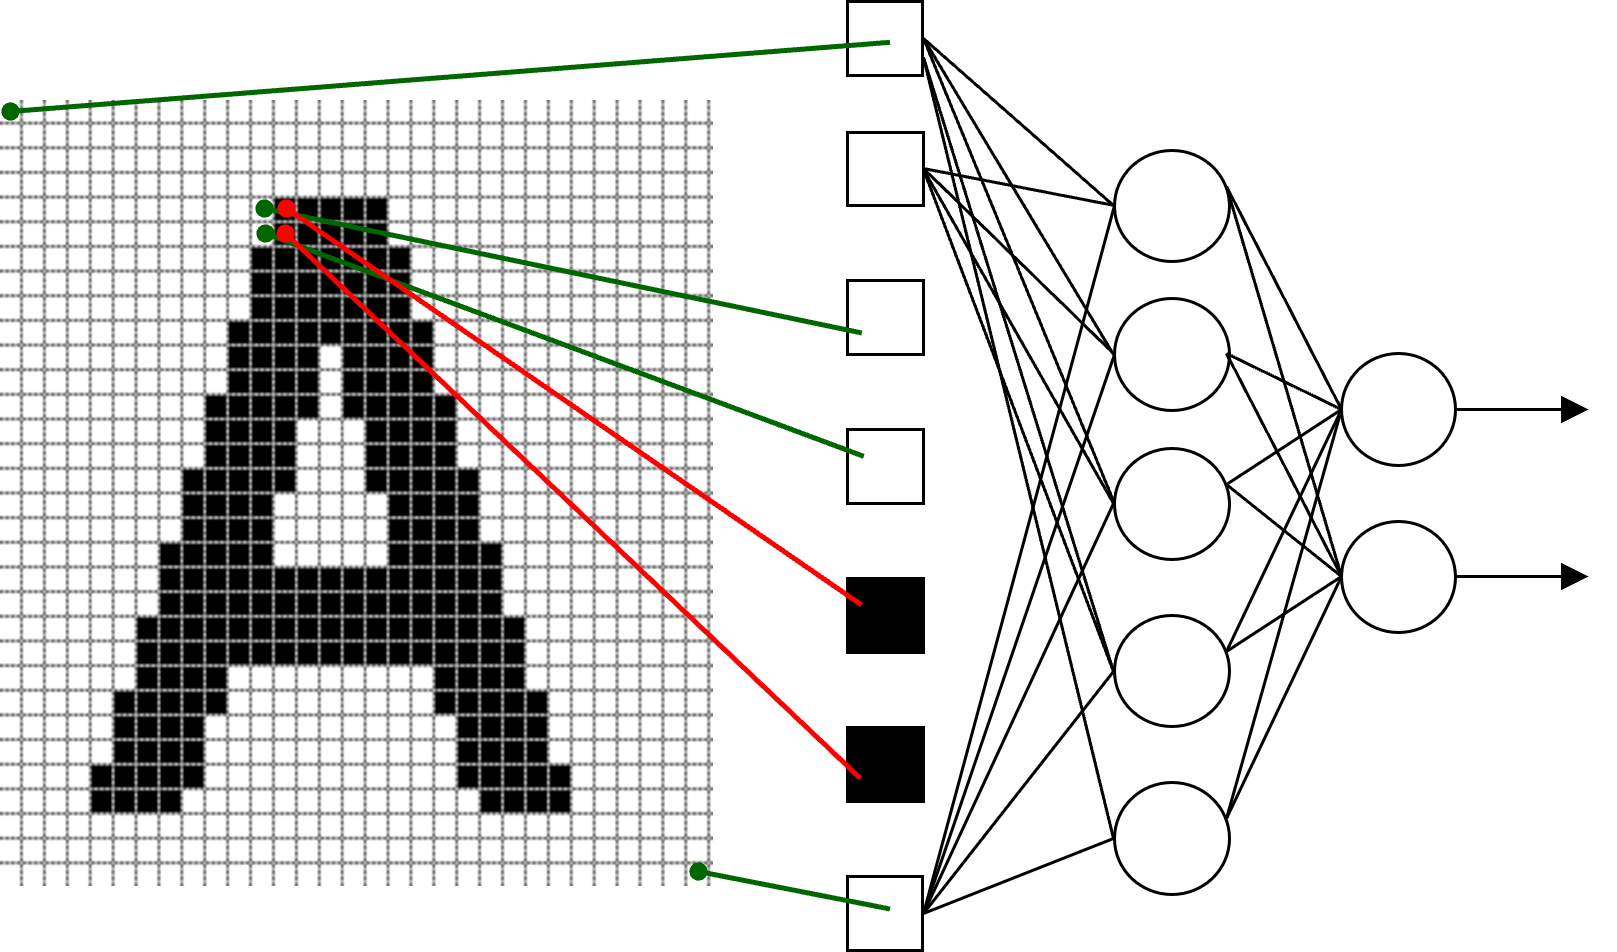
\includegraphics[width=1.0\textwidth,height=0.7\textheight,keepaspectratio]{images/cnn/nn_3.png}
    \end{figure}

\framebreak

    \begin{itemize}
        \item Little or no invariance to shifting, scaling, and other forms of distortion
    \end{itemize}

    \begin{figure}
    \centering
    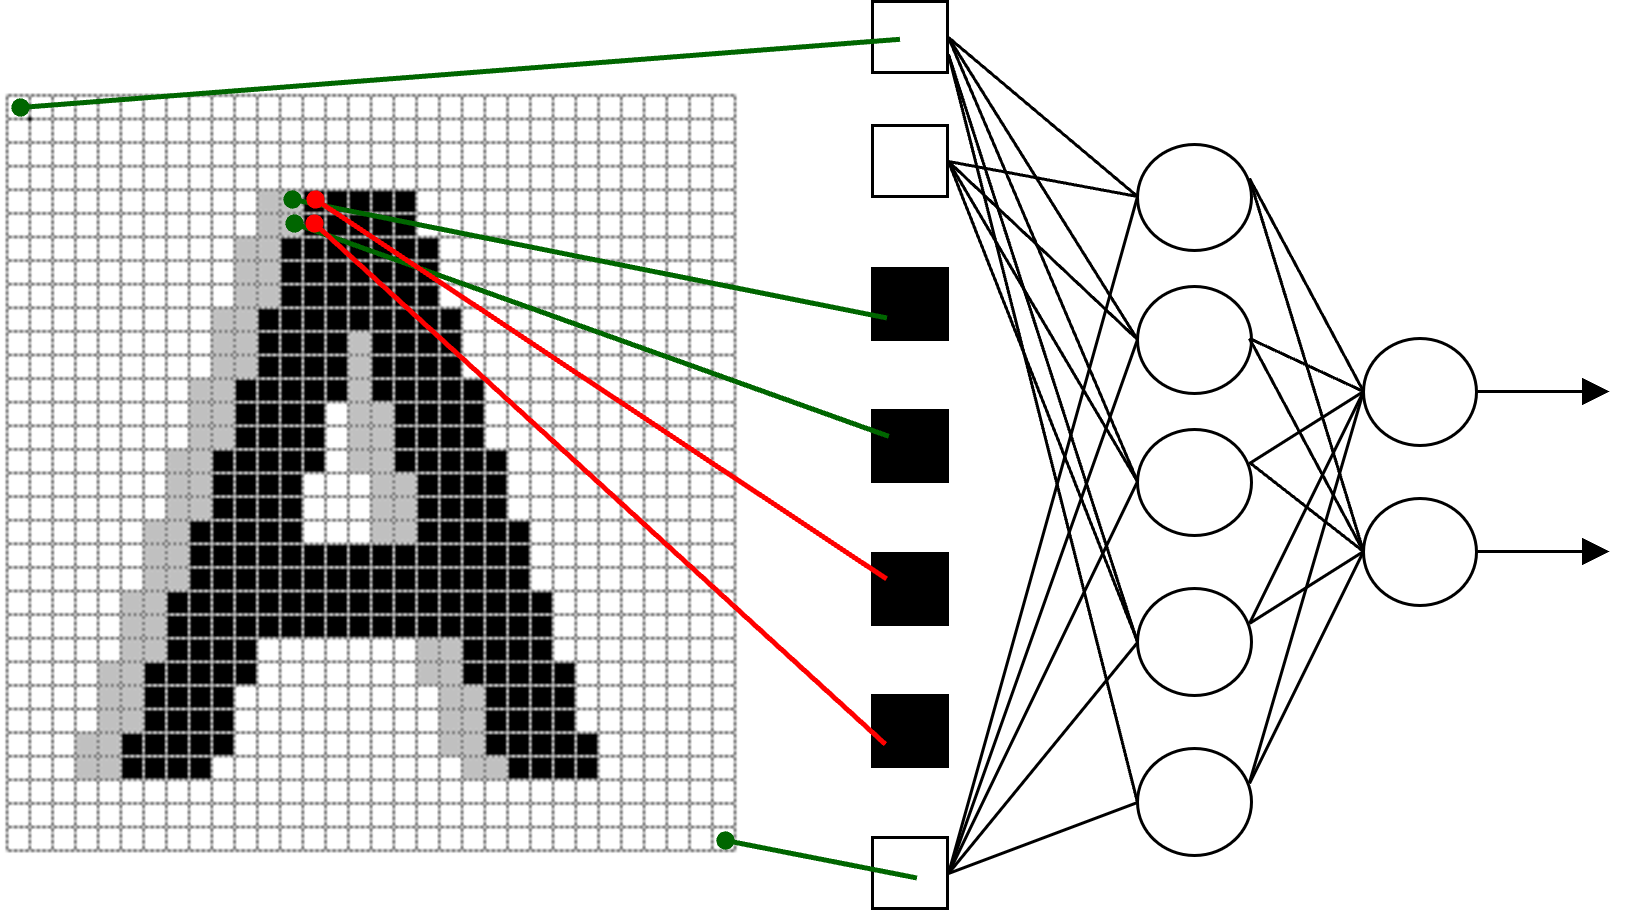
\includegraphics[width=1.0\textwidth,height=0.7\textheight,keepaspectratio]{images/cnn/nn_4.png}
    \end{figure}

\framebreak

    \begin{itemize}
        \item The topology of the input data is completely ignored
        \item For a $32 \times 32$ image, we have
        \begin{itemize}
            \item Black and white patterns: $2^{32*32} = 2^{1024}$
            \item Grayscale patterns: $256^{32*32} = 256^{1024}$
        \end{itemize}
    \end{itemize}

    \begin{figure}
    \centering
    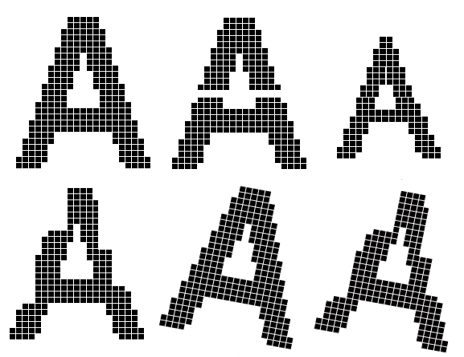
\includegraphics[width=1.0\textwidth,height=0.6\textheight,keepaspectratio]{images/cnn/nn_5.png}
    \end{figure}

\end{frame}

\begin{frame}
    \begin{center}
        We need something smarter: \\
        \LARGE \textbf{Convolution!}
    \end{center}
\end{frame}

\begin{frame}{Convolutional Neural Networks (CNNs)}
    \begin{figure}
        \centering
        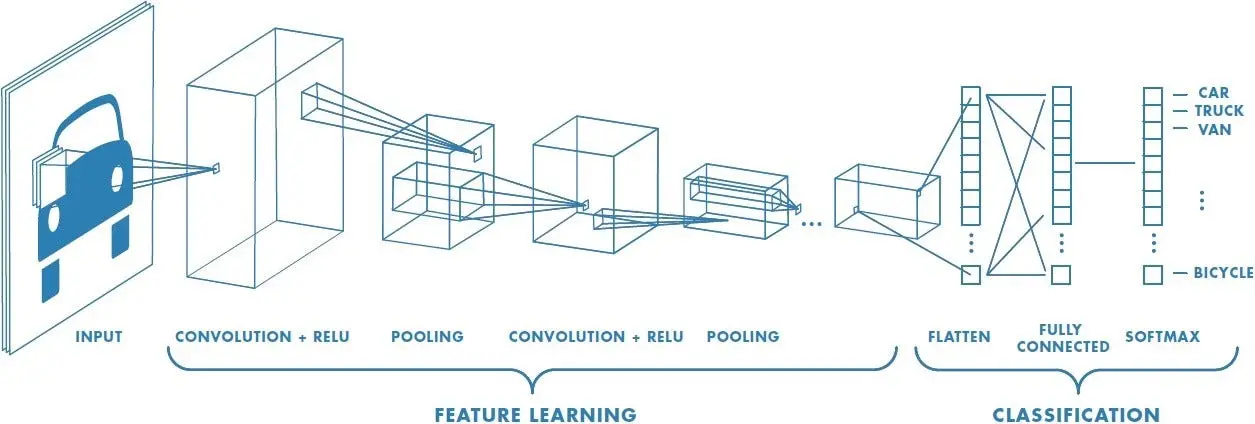
\includegraphics[width=1.0\textwidth,height=0.9\textheight,keepaspectratio]{images/cnn/cnn-architecture.png}
    \end{figure}

$$z = W * x_{i,j} = \sum_{a=0}^{m-1}\sum_{b=0}^{n-1} W_{ab}x_{(i+a)(j+b)}$$

\end{frame}

\begin{frame}[allowframebreaks]{What is Convolution?}
    \begin{itemize}
        \item A way to process local areas of the image
        \item Slide a small filter (kernel) over the image
        \item At each step, do element-wise multiply and sum
        \item Outputs a feature map (like a filtered image)
    \end{itemize}
    \begin{figure}
        \centering
        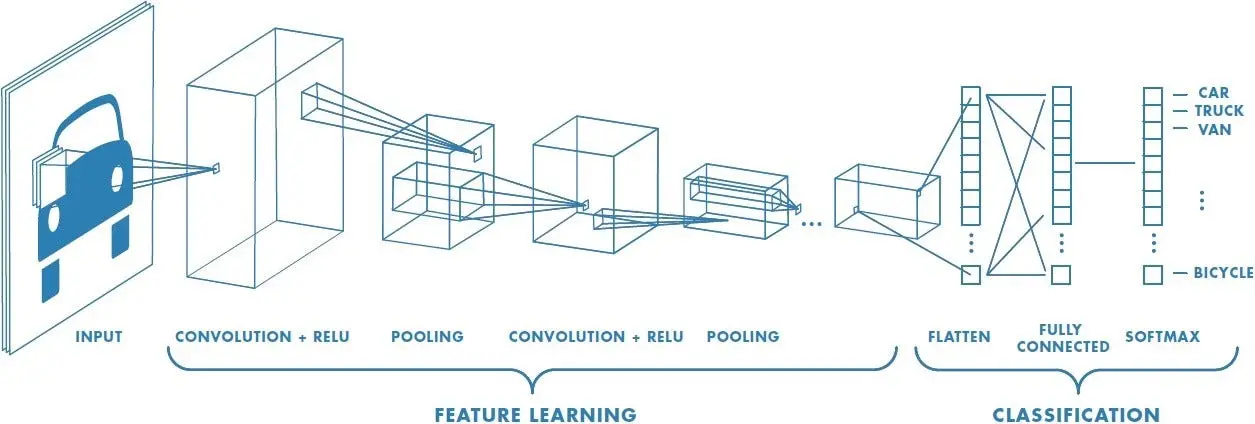
\includegraphics[width=0.9\textwidth,keepaspectratio]{images/cnn/cnn-architecture.png}
    \end{figure}
\end{frame}